\documentclass{beamer}

\usepackage[utf8]{inputenc}
\usepackage{ctex}

\usepackage{graphicx}
\usepackage{subcaption}

\usepackage{amsmath}
\usepackage{algorithm}
\usepackage{algpseudocode}



\graphicspath{ {images/} }

%\usetheme{albatross}
\usetheme{Madrid}
\usecolortheme{beaver}
%\usetheme{Antibes}


%\title[侦测隐藏敌人状态]{使用贝叶斯方法探测隐藏敌人状态 }
\title{使用贝叶斯方法探测隐藏敌人状态 }
\author{卓越羿}
\institute[SICNU]{四川师范大学数学与软件科学学院}
\date{2018}

\begin{document}

\frame{\titlepage}

\begin{frame}

\frametitle{战斗的概率模型}

给定友军和敌军,战斗被期望在它们“之间”发生,如何建模?

利用一个朴素贝叶斯分类器的“难以分类水平”定义“冲突水平”,再结合一个距离因子。

$$
P(x,y) \propto sigm(t (P_\text{ally}(x,y) (1-P_\text{ally}(x,y)) - \theta_0)) sigm(t(-\min_{u} distance + \theta_1))
$$

$$
P_\text{ally}(x,y) = \frac{
N(x\mid \mu^A_X ,\sigma^A_X) N(y \mid \mu^A_Y, \sigma^A_Y)
}{
N(x \mid \mu^A_X , \sigma^A_X) N(y \mid \mu^A_Y , \sigma^A_Y) + 
N(x \mid \mu^E_X , \sigma^E_X) N(y \mid \mu^E_Y , \sigma^E_Y)
}
$$


\end{frame}

\begin{frame}
\frametitle{葛底斯堡战役}

\begin{figure}[htb]
  \begin{subfigure}[b]{0.26\linewidth}
    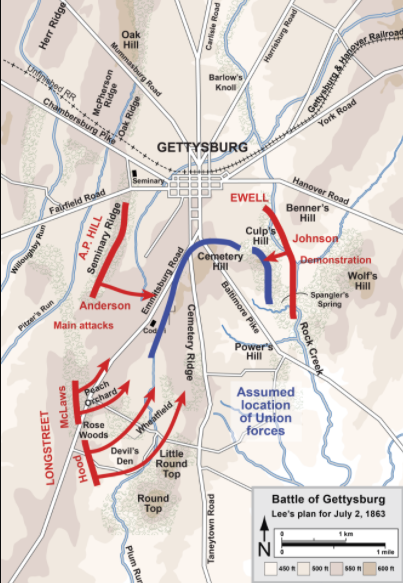
\includegraphics[width=\linewidth]{gettysburg-map.png}
    \caption{葛底斯堡战役第二天的战场示意图}
  \end{subfigure}
  \begin{subfigure}[b]{0.26\linewidth}
    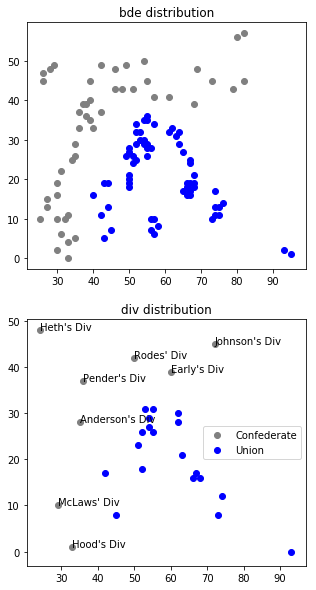
\includegraphics[width=\linewidth]{gettysburg-model.png}
    \caption{旅/师级单位位置坐标}
  \end{subfigure}
  \label{fig:gettysburg}
\end{figure}

\end{frame}

\begin{frame}

\frametitle{模型在葛底斯堡数据上的效果}

\begin{figure}[htb]
  \centering
  \begin{subfigure}[b]{0.49\linewidth}
    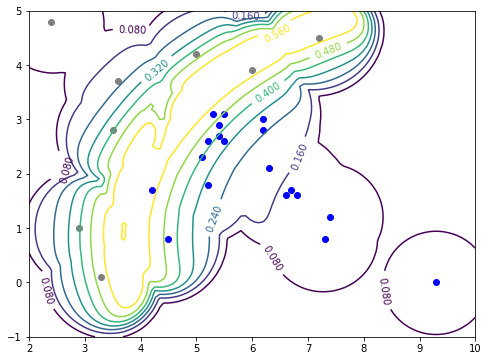
\includegraphics[width=\linewidth]{gettysburg-forward.png}
    \caption{未标准化的战役发生概率}
  \end{subfigure}
  \begin{subfigure}[b]{0.49\linewidth}
    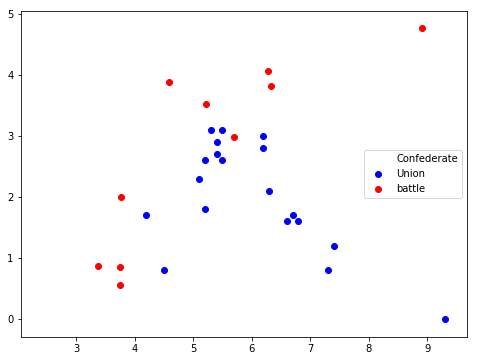
\includegraphics[width=\linewidth]{gettysburg-sample.png}
    \caption{一次采样结果+友军位置构成的模型所用数据}
  \end{subfigure}
  \caption{正向生成模型与一次采样结果}
  \label{fig:gettysburgTwo}
\end{figure}

\end{frame}

\begin{frame}

\frametitle{主要使用方法:最大后验点估计}

使用梯度上升法解决最大化问题$max_Z P(Z,D)$。下图展示了使用均匀先验(最大似然估计)和给右上角偏好
的后验点估计结果。点估计不是很有用,因为不能考虑估计的精度,也不能估计我最感兴趣的存在密度,
不过这里计算的梯度是后面两个方法的基础。

\begin{figure}[htb]
  \begin{subfigure}[b]{0.49\linewidth}
    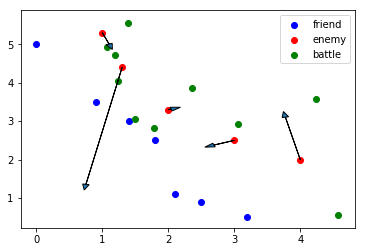
\includegraphics[width=0.6\linewidth]{MAP1.png}
    \caption{均匀先验下的MAP}
  \end{subfigure}
  \begin{subfigure}[b]{0.49\linewidth}
    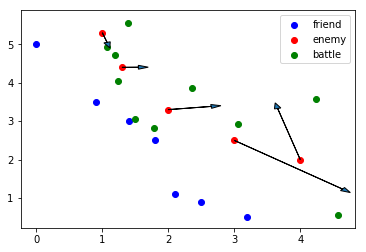
\includegraphics[width=0.6\linewidth]{MAP2.png}
    \caption{对角先验下的MAP}
  \end{subfigure}
\end{figure}

\end{frame}

\begin{frame}

\frametitle{主要使用方法:马尔科夫链蒙特卡洛(MCMC)}

这里描述的概率模型比较复杂,精确后验$P(Z \mid D) = \frac{P(D \mid Z)P(Z)}{P(D)}$中分子两项
已被正向模型确定,但分母$P(D) = \int_Z P(Z,D)$难以计算。或者就是知道这个值,计算分布的
其他参数也比较困难。若能直接从后验分布中采样,则以其一组样本,无论是估计这个值,直接当做后验分布
还是直接估计分布的参数都带来方便。

MCMC设法利用正向模型直接给出的联合概率$P(Z,D)$之比率(正好消掉$P(D)$)来构造一个随机游走来获取后验分布的样本。
两个隐变量/随机参数取值$P(Z_1,D),P(Z_2,D)$中,值更大者游走到的概率越大。随机游走的稳态分布被保证为精确后验分布。

如经典的Metropolis-Hastings算法中,给定初始值$Z_0$后,每步根据当前$Z_t$
随机抽一个试探点$\bar{Z_t}$(如$\bar{Z_t} \sim N(Z_t,1)$,以$Z_t$为中心。),
以$\min(1,P(\bar{Z_t},D)/P(Z_t,D))$为概率转移到试探点$Z_t$。

\end{frame}

\begin{frame}


\frametitle{MCMC:哈密顿蒙特卡洛(HMC)}

HMC不需要指定proposal分布而是由梯度指导游走,效率更高。

\begin{algorithm}[H]

\tiny

\caption{哈密顿蒙特卡洛采样}
\begin{algorithmic}[1]
\Procedure{HMC}{$\theta_0,\epsilon,L,step$} \Comment{$L$ ,$\epsilon$ 是 leap-frog过程的参数}
    \For{$i$ in $1:step$}
        \State $r_0 \sim N(0,I)$
        \State $\theta_i \gets \tilde{\theta} \gets \theta_{i-1}$
        \State $\tilde{r} \gets r_0$
        \For{$l$ in $1:L$} \Comment{leap-frog过程}
            \State $\tilde{r} \gets \tilde{r} + (\epsilon/2) \nabla_\theta P(X,\theta)|_{\tilde{\theta}}$
            \State $\tilde{\theta} \gets \tilde{\theta} + \epsilon \tilde{r}$
            \State $\tilde{r} \gets \tilde{r} + (\epsilon/2) \nabla_\theta P(X,\theta)|_{\tilde{\theta}}$
        \EndFor
        \State $\alpha \gets \min \left\{ 1, \frac{\exp(P(x,\tilde{\theta})-\frac{1}{2}\tilde{r}\cdot\tilde{r})}{\exp(P(x,\theta_{i-1})-\frac{1}{2}r_0\cdot r_0)} \right\}$  \Comment{接受率,转移概率}
        \State $u \sim \mathrm{Uniform}(0,1)$
        \If{$u \le \alpha$}
            \State $\theta^i \gets \tilde{\theta}$
        \EndIf
    \EndFor
    \State \Return $\theta$
\EndProcedure
\end{algorithmic}
\label{alg:hmc}
\end{algorithm}

\end{frame}

\begin{frame}

\frametitle{主要使用方法:变分推断}

利用正态分布族近似精确后验分布,近似优劣以降低KL散度为准:

$$
KL(q||p) = E_q \left( \log \frac{q(\theta \mid \mu,\omega)}{p(\theta \mid x)} \right)
$$

$p(\theta \mid x)$无法计算,转而等价地最大化置信下界$ELBO$

$$
\mathrm{ELBO} = E_q (\log p(x,\theta)) - E_q(\log q(\theta)) 
$$

$E_q(\cdot)$可用蒙特卡洛积分近似计算

\end{frame}

\begin{frame}
\frametitle{变分推断算法:自动微分变分推断(ADVI)}

\begin{algorithm}[H]

\tiny

\caption{自动微分变分推断(平均场,不考虑变换)}
\begin{algorithmic}[1]
\Procedure{ADVI}{$\mathbf{\mu},\mathbf{\omega},lr,M,step$}  \Comment{$\mathbf{\mu},\mathbf{\omega}$ 是初始值,$M$是随机积分采样个数}
    \For{$s$ in $1:step$}
        \State $\hat{\nabla}_\mathbf{\mu} \gets \mathbf{0}$
        \State $\hat{\nabla}_\mathbf{\omega} \gets \mathbf{0}$
        \For{$i$ in $1:M$} 
            \State $\mathbf{\eta} \sim N(\mathbf{0},\mathbf{I}) $ \Comment{从多元标准正态分布中采样,下同}
            \State $\hat{\theta} \gets (\mathbf{\eta} * \exp(\mathbf{\omega})) + \mathbf{\mu}$ \Comment{$*$即按元素对应相乘}
            \State $\hat{\nabla}_\mathbf{\mu} \gets \hat{\nabla}_\mathbf{\mu} + (\nabla_\theta \log p(x,\theta)|_{\hat{\theta}})$
            \State $\hat{\nabla}_\mathbf{\omega} \gets \hat{\nabla}_\mathbf{\omega} + \hat{\nabla}_\mu * \mathbf{\eta}$
        \EndFor
        \State $\hat{\nabla}_{\mathbf{\mu}} \gets \hat{\nabla}_{\mathbf{\mu}} / M$
        \State $\hat{\nabla}_{\mathbf{\omega}} \gets (\hat{\nabla}_\mathbf{\omega} / M) * \exp(\mathbf{\omega}) + \mathbf{1}$
        \State $\mathbf{\mu} \gets \mathbf{\mu} + lr \hat{\nabla}_{\mathbf{\mu}}$
        \State $\mathbf{\omega} \gets \mathbf{\mu} + lr \hat{\nabla}_{\mathbf{\omega}}$
    \EndFor 
    \State \Return $\mathbf{\mu},\mathbf{\omega}$
\EndProcedure
\end{algorithmic}
\label{alg:advi}
\end{algorithm}

\end{frame}

\begin{frame}
\frametitle{应用:敌对单位位置后验分布估计}

\begin{figure}[htb]
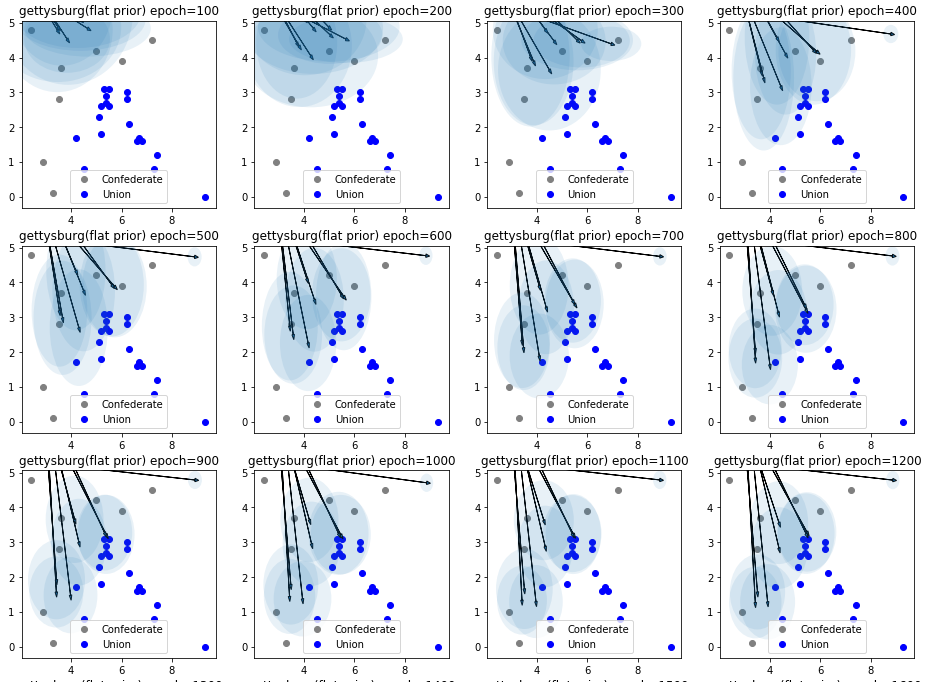
\includegraphics[width=0.8\linewidth]{gettysburg-point-small.png}
\label{fig:gettysburgInit}
\end{figure}



\end{frame}

\begin{frame}
\frametitle{应用:敌对单位存在概率密度估计}

采用正态分布族的变分推断的一大好处就是计算特定敌军单位在特定区域的后验概率十分方便。
从而可以直接计算出任意矩形区域$[x,x+dx]\times[y,y+dy]$中存在任意敌军单位的概率:

\begin{align*}
pe(x,y,dx,dy) = 1-
\prod_i^{N_E}
(1-
& ((\Phi((x + dx - \mu_{X^E_i})/\sigma_{X^E_i}) - \Phi((x - \mu_{X^E_i})/\sigma_{X^E_i})) \\
&  (\Phi((y + dy - \mu_{Y^E_i})/\sigma_{Y^E_i}) - \Phi((y - \mu_{Y^E_i})/\sigma_{Y^E_i})))
)
\end{align*}

%而$\mu_{X^E_i}$是第$i$个敌人的近似后验分布的正态期望参数,另外几个类似。
%这种话就不写在ppt里了,临时解释就是。

从而近似地计算出存在密度:

$$
pe(x,y) = pe(x-\epsilon,y-\epsilon,2\epsilon,2\epsilon)/(4 \epsilon^2)
$$

\end{frame}

\begin{frame}
\frametitle{葛底斯堡战役数据的存在推断收敛过程}

\begin{figure}[htb]
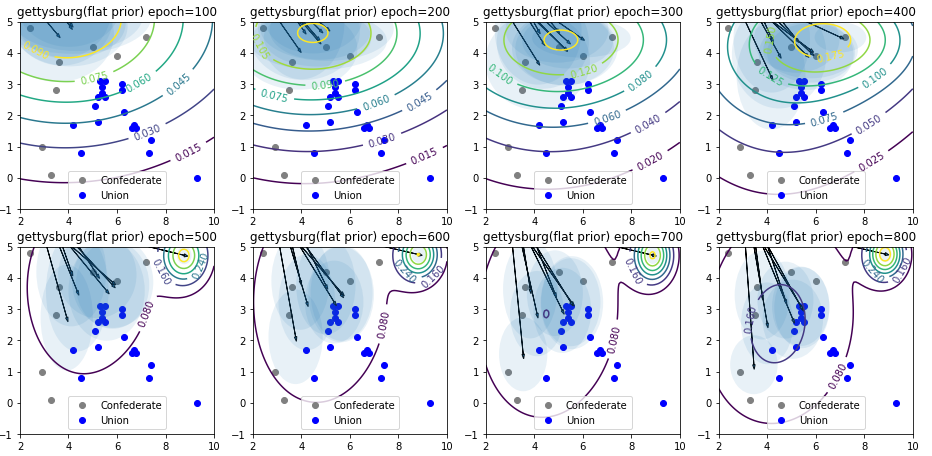
\includegraphics[width=0.99\linewidth]{gettysburg-init-beamer.png}
\label{fig:gettysburgInit}
\end{figure}


\end{frame}

\begin{frame}

\frametitle{变体:考虑规模效应}

葛底斯堡战役例子里各个单位的兵力和战斗力显然不是一致的,南方邦联军的一个师肯定比联邦强。
这里设定成规模越大,它的“等效距离”越短(6000兵力的师的“等效距离”看成之前的距离一样),
同时在计算贝叶斯分类器参数(如类均值$\mu^S_Z$)时的权重更高。



\begin{figure}[htb]
  \centering
  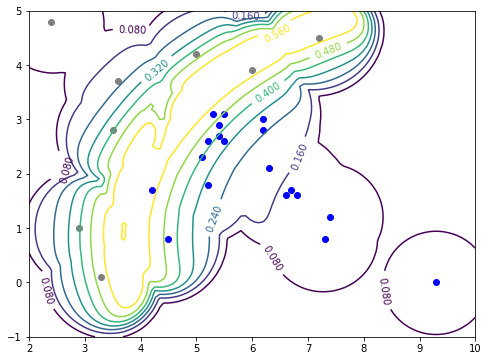
\includegraphics[width=0.3\linewidth]{gettysburg-forward.png}
  \caption{带规模效应模型的正向概率}
\end{figure}

迭代图太长而且没有前面收敛那么早所以不插到这,\href{gettysburg2.html}{notebook}。

\end{frame}

\begin{frame}

\frametitle{变体:移动侦测}

原来的模型的隐变量只有$Z^E_i$,将其变为表示期初点与期末点两个隐变量$Z^E_i(0),Z^E_i(1)$。
再假定单位都在均匀运动$Z^E_i(t) =(1-t) Z^E_i(0) + t Z^E_i(1) \quad t \in [0,1]$。就可以
把模型改造成可以推断运动,当然这么轻易的改效果不是很好。

\begin{figure}[htb]
  \begin{subfigure}[b]{0.49\linewidth}
    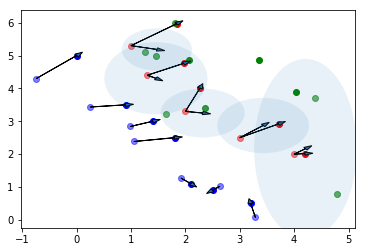
\includegraphics[width=0.6\linewidth]{bkeu.png}
    \caption{运动推断:$t=0$已知而$t=1$未知}
  \end{subfigure}
  \begin{subfigure}[b]{0.49\linewidth}
    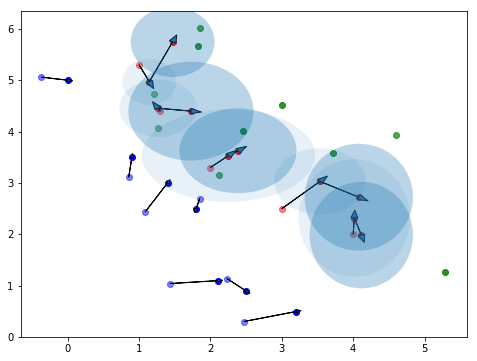
\includegraphics[width=0.6\linewidth]{bueu.png}
    \caption{运动推断:$t=0$与$t=1$时敌人位置都未知}
  \end{subfigure}
\end{figure}


\end{frame}

\begin{frame}

\frametitle{其他扩展}

本文除了考虑了移动侦测,考虑规模效应的变体。还考虑设置不同先验,设置不同初始值,各种数据形态检验模型有效性。
也考虑了比较这个模型以外的几个模型的效果。也讨论了哈密顿蒙特卡洛实现等。具体内容见原文。

\begin{figure}[htb]
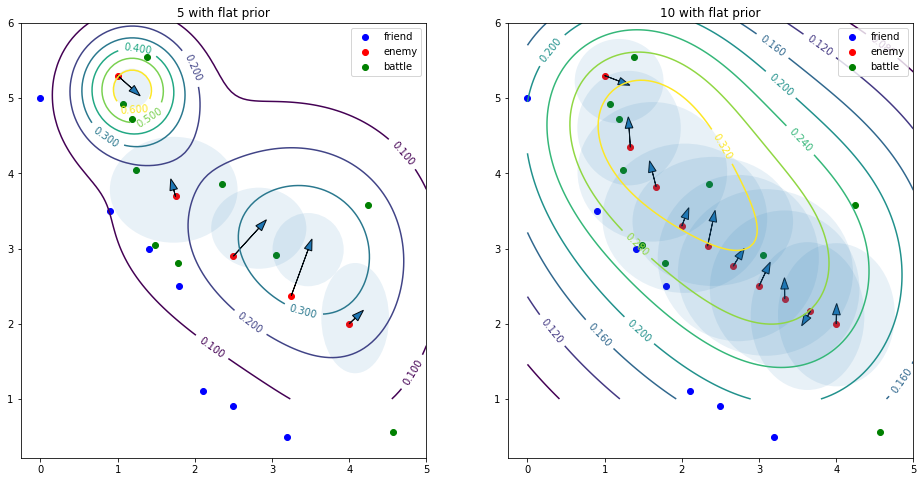
\includegraphics[width=0.7\linewidth]{exist_density.png}
\label{fig:gettysburgInit}
\end{figure}

\end{frame}

\begin{frame}

\frametitle{问题时间}

\begin{figure}[htb]

\includegraphics[width=0.9\linewidth]{elder.png}
\end{figure}

\end{frame}

\end{document}